\chapter{Relacje równoważności i zbiory ilorazowe}\label{ch:equivalence}

\section{Dlaczego sama równość nie wystarcza?}\label{sec:eq-motivation}
Równość $a=b$ jest najbardziej rygorystycznym sposobem uznania dwóch
obiektów za nierozróżnialne. W matematyce często chcemy jednak pomijać
pewien rodzaj różnicy. Na przykład liczby $2$ i $7$ nie są równe,
ale przy dzieleniu przez $5$ dają tę samą resztę. Dwa napisy mogą się
różnić kolejnością liter, lecz mieć tę samą długość. Dwa ułamki
$1/2$ i $2/4$ są różnymi parami liczb, chociaż opisują tę samą
liczbę wymierną. Chcemy opisać wspólny mechanizm takich utożsamień.

W rozdziale~\ref{ch:relations} poznaliśmy zwrotność, symetrię i
przechodniość. Łącznie są one dokładnie własnościami pozwalającymi
rozsądnie grupować obiekty, które w wybranym znaczeniu uważamy za
równoważne. Najpierw pokażemy to na przykładach, a potem sformalizujemy.

\begin{definicja}[Relacja równoważności]\label{def:equivalence}
Niech $X$ będzie zbiorem, a $E\subseteq X\times X$ relacją.
Nazywamy $E$ \emph{relacją równoważności na $X$}, jeśli
\begin{enumerate}[label=(\roman*)]
\item dla każdego $x\in X$ zachodzi $xEx$ (zwrotność);
\item dla wszystkich $x,y\in X$, z $xEy$ wynika $yEx$ (symetria);
\item dla wszystkich $x,y,z\in X$, z $xEy$ i $yEz$ wynika $xEz$
(przechodniość).
\end{enumerate}
Najczęściej zapisujemy $x\sim y$ zamiast $xEy$.
\end{definicja}

\begin{przyklad}[Równość i relacja całkowita]
Na dowolnym zbiorze $X$ relacja $x\sim y\iff x=y$ jest
równoważnością: każdy element jest równy samemu sobie, równość
można odwrócić i składać. Relacja $x\sim y$ dla \emph{każdych}
$x,y\in X$ także jest równoważnością. W pierwszym przypadku
niczego nie utożsamiamy, w drugim utożsamiamy wszystkie elementy.
Obie relacje są równoważnościami również dla $X=\varnothing$.
\end{przyklad}

\begin{przyklad}[Te same reszty z dzielenia]\label{ex:eq-congruence}
Ustalmy liczbę naturalną $m\ge1$. Na $\Z$ określmy
\[
 a\sim_m b\quad\Longleftrightarrow\quad
 m\mid(a-b),
\]
gdzie $m\mid t$ znaczy, że istnieje $k\in\Z$ z $t=mk$.
Zwrotność wynika z $a-a=m\cdot0$. Jeśli $a-b=mk$, to
$b-a=m(-k)$, zatem zachodzi symetria. Jeśli
$a-b=mk$ oraz $b-c=m\ell$, to dodając równości dostajemy
$a-c=m(k+\ell)$; to dowodzi przechodniości.
Dla $m=5$ liczby $2,7,-3,12$ są równoważne. Dla $m=1$
wszystkie liczby całkowite są równoważne.
\end{przyklad}

\begin{przyklad}[Bliskość nie jest równoważnością]
Na $\R$ ustalmy $xRy\iff |x-y|<1$. Relacja jest zwrotna
i symetryczna, ale nieprzechodnia: $0R\frac34$ i
$\frac34R\frac32$, natomiast $0\not R\frac32$.
Sama intuicja podobieństwa nie wystarcza, jeśli nie można
przenosić jej przez pośrednie obiekty.
\end{przyklad}

\section{Klasy równoważności i ich podstawowe własności}
\label{sec:eq-classes}
\begin{definicja}[Klasa równoważności]\label{def:eq-class}
Niech $X$ będzie zbiorem, a $\sim$ relacją równoważności na $X$.
Dla $x\in X$ \emph{klasą równoważności elementu $x$} nazywamy
\[
 [x]_{\sim}:=\{y\in X:y\sim x\}.
\]
Gdy relacja jest jasna, piszemy krótko $[x]$. Zbiór
wszystkich klas równoważności oznaczamy
\[
 X/{\sim}:=\{[x]_{\sim}:x\in X\}
\]
i nazywamy \emph{zbiorem ilorazowym} zbioru $X$ przez $\sim$.
Każdy element $X/{\sim}$ jest sam w sobie podzbiorem $X$.
\end{definicja}

\begin{uwaga}[Istnienie zbioru ilorazowego, także dla pustego $X$]
Każda klasa $[x]_{\sim}$ jest podzbiorem $X$, więc
$X/{\sim}\subseteq\mathcal P(X)$. Aby otrzymać iloraz jako
zbiór w ZF, można wyciąć z już istniejącego zbioru
$\mathcal P(X)$ te i tylko te podzbiory $C$, dla których
istnieje $x\in X$ spełniający
$\forall y\in X\,(y\in C\iff y\sim x)$.
To jest zastosowanie schematu wyróżniania, a nie
nieograniczonego tworzenia zbioru z warunku.
Jeśli $X=\varnothing$, jedyna relacja na $X$ jest pusta,
nie istnieje żaden $x\in X$, a więc $X/{\sim}=\varnothing$.
W przypadku niepustego $X$ każda klasa jest niepusta,
ale nie oznacza to, że sam zbiór ilorazowy ma jeden element:
liczba klas zależy od przyjętej relacji.
\end{uwaga}



\begin{uwaga}[Element, singleton i klasa]
Dla $x\in X$ mamy trzy potencjalnie różne obiekty: $x$,
$\{x\}$ oraz $[x]$. Zwrotność zapewnia $x\in[x]$,
a więc $[x]\ne\varnothing$, lecz nie musi zachodzić
$[x]=\{x\}$. Na przykład w relacji kongruencji modulo $5$
klasa $[2]$ zawiera nieskończenie wiele liczb całkowitych.
\end{uwaga}

\begin{twierdzenie}[Kiedy dwie klasy są równe?]\label{thm:class-equality}
Niech $X$ będzie zbiorem, a $\sim$ relacją równoważności na $X$.
Dla dowolnych $x,y\in X$ następujące warunki są równoważne:
\begin{enumerate}[label=(\roman*)]
\item $x\sim y$;
\item $[x]=[y]$;
\item $[x]\cap[y]\ne\varnothing$.
\end{enumerate}
\end{twierdzenie}
\begin{proof}
Najpierw załóżmy $x\sim y$. Aby wykazać $[x]\subseteq[y]$,
wybierzmy dowolny $z\in[x]$. Definicja klasy daje $z\sim x$.
Z przechodniości $z\sim x$ i $x\sim y$ wynika $z\sim y$,
a więc $z\in[y]$. W drugą stronę, jeśli $z\in[y]$, to
$z\sim y$; z symetrii $x\sim y$ mamy $y\sim x$.
Przechodniość daje $z\sim x$, zatem $z\in[x]$.
Pokazaliśmy oba zawierania, więc $[x]=[y]$.

Jeżeli $[x]=[y]$, to dzięki zwrotności $x\in[x]$,
a zatem $x\in[x]\cap[y]$. Przecięcie jest niepuste.

Wreszcie załóżmy $[x]\cap[y]\ne\varnothing$.
Istnieje wtedy $z\in X$ należący do obu klas.
Oznacza to $z\sim x$ i $z\sim y$.
Z symetrii pierwszej relacji wynika $x\sim z$.
Łącząc $x\sim z$ z $z\sim y$, otrzymujemy
$x\sim y$ przez przechodniość. Zamknęliśmy ciąg implikacji.
\end{proof}

\begin{wniosek}[Klasy nie przecinają się częściowo]\label{cor:eq-disjoint}
Niech $X$ będzie zbiorem, a $\sim$ relacją równoważności na $X$.
Dla dowolnych $x,y\in X$ klasy $[x]$ i $[y]$
są albo rozłączne, albo równe. Ponadto
\[
 X=\bigcup_{x\in X}[x].
\]
\end{wniosek}
\begin{proof}
Jeśli przecięcie klas jest niepuste, to na mocy
Twierdzenia~\ref{thm:class-equality} klasy są równe.
Daje to pierwszą tezę. Każda klasa jest podzbiorem $X$,
więc ich suma zawiera się w $X$. Odwrotnie, dowolny
$x\in X$ należy do $[x]$ przez zwrotność. Zatem
$x$ należy do sumy wszystkich klas. Stąd równość.
Gdy $X=\varnothing$, prawa strona jest pustą sumą i nadal
otrzymujemy równość.
\end{proof}

\begin{przyklad}[Kongruencje modulo $3$]
Na $\Z$ przy relacji $\sim_3$ mamy dokładnie trzy różne klasy:
\[
 [0]=\{3k:k\in\Z\},\quad
 [1]=\{3k+1:k\in\Z\},\quad
 [2]=\{3k+2:k\in\Z\}.
\]
Każda liczba całkowita należy do dokładnie jednej z nich:
dzieląc ją przez $3$ otrzymujemy dokładnie jedną z reszt
$0,1,2$. Klasy $[3]$ i $[0]$ nie są dwiema różnymi klasami;
ponieważ $3\sim_3 0$, są tym samym podzbiorem $\Z$.
\end{przyklad}

\begin{przyklad}[Przykład geometryczny]
Na płaszczyźnie $\R^2$ ustalmy
$(x,y)\sim(u,v)\iff y=v$. Zwrotność, symetria i
przechodniość wynikają z tych własności równości drugiej
współrzędnej. Klasa punktu $(x_0,y_0)$ ma postać
$\{(x,y_0):x\in\R\}$, czyli jest prostą poziomą.
Zbiór ilorazowy składa się z \emph{prostych poziomych},
a nie z pojedynczych punktów płaszczyzny.
\end{przyklad}

\begin{center}
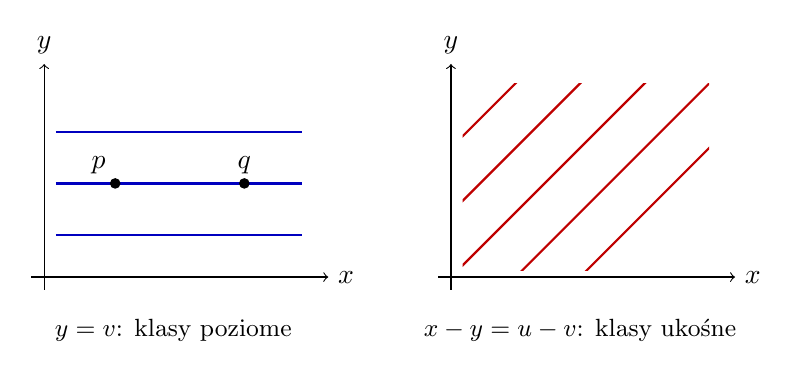
\begin{tikzpicture}[x=0.82cm,y=0.82cm]
  \begin{scope}[shift={(0,0)}]
    \draw[->] (-.2,0)--(4.4,0) node[right] {$x$};
    \draw[->] (0,-.2)--(0,3.3) node[above] {$y$};
    \foreach \h in {.65,1.45,2.25} {
      \draw[blue!75!black,thick] (.18,\h)--(4.0,\h);
    }
    \filldraw (1.1,1.45) circle (1.7pt) node[above left] {$p$};
    \filldraw (3.1,1.45) circle (1.7pt) node[above] {$q$};
    \node[font=\small,anchor=north] at (2.0,-.5) {$y=v$: klasy poziome};
  \end{scope}
  \begin{scope}[shift={(6.3,0)}]
    \draw[->] (-.2,0)--(4.4,0) node[right] {$x$};
    \draw[->] (0,-.2)--(0,3.3) node[above] {$y$};
    \begin{scope}
      \clip (.18,.1) rectangle (4,3);
      \foreach \c in {-2,-1,0,1,2} {
        \draw[red!75!black,thick] (-.8,{-.8+\c})--(5,{5+\c});
      }
    \end{scope}
    \node[font=\small,anchor=north] at (2,-.5) {$x-y=u-v$: klasy ukośne};
  \end{scope}
\end{tikzpicture}

{\small Po lewej klasy relacji $(x,y)\sim(u,v)\iff y=v$;
po prawej klasy \emph{innej} relacji
$(x,y)\approx(u,v)\iff x-y=u-v$.
Na każdym panelu różne klasy nie mają punktów wspólnych.}
\end{center}


\begin{uwaga}[Dlaczego czerwone i niebieskie proste opisują różne relacje?]
Na rysunku powyżej dwie poziome proste nie przecinają się,
ponieważ stanowią dwie różne klasy \emph{tej samej} relacji
„mieć jednakową drugą współrzędną”. Czerwone proste
są klasami innej relacji, „mieć jednakową różnicę współrzędnych”.
Czerwona i niebieska prosta mogą się przeciąć i nie narusza to
Twierdzenia~\ref{thm:class-equality}: twierdzenie o rozłączności
różnych klas dotyczy klas \emph{jednej ustalonej} relacji.
\end{uwaga}

\section{Podziały zbioru i równoważności}\label{sec:eq-partition}
\begin{definicja}[Podział zbioru]\label{def:partition}
Niech $X$ będzie zbiorem. \emph{Podziałem $X$} nazywamy
rodzinę $\mathcal D$ podzbiorów $X$ spełniającą:
\begin{enumerate}[label=(\roman*)]
\item każdy $D\in\mathcal D$ jest niepusty;
\item jeśli $D,E\in\mathcal D$ i $D\ne E$, to
$D\cap E=\varnothing$;
\item $\bigcup_{D\in\mathcal D}D=X$.
\end{enumerate}
Dla $X=\varnothing$ rodzinę pustą uznajemy za podział;
co więcej, jest ona jedynym podziałem pustego zbioru: każdy
blok musiałby być niepustym podzbiorem $\varnothing$, co jest niemożliwe.
Elementy $\mathcal D$ nazywamy \emph{blokami podziału}.
\end{definicja}

\begin{twierdzenie}[Równoważności i podziały]\label{thm:eq-partition}
Niech $X$ będzie dowolnym zbiorem.
\begin{enumerate}[label=(\roman*)]
\item Każda relacja równoważności $\sim$ na $X$ wyznacza
podział $\mathcal D_{\sim}:=X/{\sim}$.
\item Każdy podział $\mathcal D$ zbioru $X$ wyznacza relację
$\sim_{\mathcal D}$, określoną przez
\[
 x\sim_{\mathcal D}y\iff
 \text{istnieje }D\in\mathcal D\text{ takie, że }x,y\in D.
\]
Dla wszystkich $x,y\in X$ formuła ta określa relację
równoważności, której klasami są dokładnie bloki $\mathcal D$.
\item Przejścia opisane w (i) i (ii) są wzajemnie odwrotne:
wyznaczają jednoznaczną odpowiedniość między wszystkimi
relacjami równoważności na $X$ a wszystkimi podziałami $X$.
\end{enumerate}
\end{twierdzenie}
\begin{proof}
(i) Z definicji klasy $[x]\subseteq X$, a zwrotność
gwarantuje $x\in[x]$, czyli klasa jest niepusta.
Wniosek~\ref{cor:eq-disjoint} mówi, że różne klasy są rozłączne
i że ich suma jest całym $X$. To są dokładnie trzy warunki
w definicji podziału.

(ii) Ponieważ $\mathcal D$ pokrywa $X$, dla każdego
$x\in X$ istnieje blok $D$ zawierający $x$.
Wtedy $x,x\in D$, więc $x\sim_{\mathcal D}x$.
Jeżeli $x,y\in D$, to także $y,x\in D$, więc zachodzi
symetria. Dla przechodniości załóżmy
$x\sim_{\mathcal D}y$ oraz $y\sim_{\mathcal D}z$.
Istnieją bloki $D,E\in\mathcal D$ takie, że
$x,y\in D$ i $y,z\in E$. W szczególności $y\in D\cap E$.
Przecięcie nie jest puste, więc z warunku rozłączności
różnych bloków musi zachodzić $D=E$. Wtedy $x,z\in D$,
zatem $x\sim_{\mathcal D}z$.

Niech teraz $D\in\mathcal D$ i $x\in D$ (taki $x$
istnieje, bo bloki są niepuste). Jeśli $y\in D$, to
$x\sim_{\mathcal D}y$, a więc $y\in[x]$.
Odwrotnie, jeżeli $y\in[x]$, to $y$ i $x$ należą do
pewnego wspólnego bloku $E$. Ponieważ $x\in D\cap E$,
wynika $E=D$, a zatem $y\in D$. Stąd $[x]=D$.
Każdy blok jest więc klasą. Odwrotnie, dla dowolnego
$x\in X$ istnieje blok $D\in\mathcal D$ zawierający $x$
(z warunku pokrycia), a pokazany argument daje $[x]=D$.
Zatem każda klasa jest blokiem, także gdy $X=\varnothing$
(wówczas oba zbiory klas i bloków są puste).

(iii) Jeśli zaczęliśmy od relacji $\sim$, to dla
$x,y\in X$ warunek przynależności do wspólnej klasy
jest równoważny $x\sim y$ na mocy
Twierdzenia~\ref{thm:class-equality}.
Odzyskujemy więc tę samą relację. Jeśli zaczęliśmy
od podziału $\mathcal D$, to (ii) pokazało, że klasy
wyznaczonej relacji są dokładnie blokami $\mathcal D$.
Odzyskujemy więc dokładnie ten sam podział.
\end{proof}

\begin{przyklad}[Wszystkie podziały trójelementowego zbioru]
\label{ex:eq-partitions-three-xliii}
Niech $X=\{a,b,c\}$. Każdy podział ma dokładnie jeden,
dwa albo trzy bloki. Przy jednym bloku istnieje tylko
$\{\{a,b,c\}\}$. Przy trzech blokach istnieje tylko
$\{\{a\},\{b\},\{c\}\}$. Przy dwóch blokach jeden ma
jeden element, a drugi dwa; otrzymujemy dokładnie
\begin{gather*}\{\{a\},\{b,c\}\},\quad \{\{b\},\{a,c\}\},\quad\{\{c\},\{a,b\}\}.\end{gather*}
Zatem wszystkich podziałów jest pięć, a na mocy
Twierdzenia~\ref{thm:eq-partition} także relacji
równoważności na $X$ jest pięć. Nie wolno tu liczyć
uporządkowanych list bloków: zamiana kolejności bloków
nie tworzy nowego podziału.
\end{przyklad}



\begin{przyklad}[Podziały skończonego zbioru]
Dla $X=\{a,b,c\}$ jednymi z możliwych podziałów są
$\{\{a\},\{b\},\{c\}\}$,
$\{\{a,b\},\{c\}\}$ oraz $\{\{a,b,c\}\}$.
Pierwszy odpowiada równości, trzeci relacji pełnej,
a drugi utożsamieniu wyłącznie elementów $a,b$.
Zwróćmy uwagę na różnicę pomiędzy zbiorem $X$ a
zbiorem jego bloków: w drugim przykładzie mamy dwa
bloki, choć zbiór $X$ ma trzy elementy.
\end{przyklad}

\section{Uogólnianie i uszczegóławianie identyfikacji}\label{sec:eq-refinement}
\begin{definicja}[Relacja drobniejsza i grubsza]
Niech $X$ będzie zbiorem. Jeżeli $E,F$ są relacjami
równoważności na $X$, to $E$ nazywamy \emph{drobniejszą} od $F$,
gdy $E\subseteq F$ jako podzbiory $X\times X$.
Oznacza to, że $E$ utożsamia nie więcej par niż $F$.
W tej samej sytuacji relację $F$ nazywamy \emph{grubszą}
od $E$.
\end{definicja}

\begin{twierdzenie}[Drobniejsza relacja ma mniejsze klasy]
\label{thm:eq-refinement}
Niech $X$ będzie zbiorem, a $E,F$ relacjami
równoważności na $X$. Wtedy $E\subseteq F$ wtedy i tylko wtedy,
gdy $[x]_E\subseteq[x]_F$ dla każdego $x\in X$.
\end{twierdzenie}
\begin{proof}
Załóżmy $E\subseteq F$. Jeśli $y\in[x]_E$, to $yEx$,
a z zawierania relacji wynika $yFx$. Zatem
$y\in[x]_F$. Udowodniliśmy zawieranie klas.

Odwrotnie, załóżmy zawieranie klas dla wszystkich $x$.
Jeśli $(x,y)\in E$, to $xEy$ i stąd
$x\in[y]_E\subseteq[y]_F$. Definicja klasy daje $xFy$,
czyli $(x,y)\in F$. To dowodzi $E\subseteq F$.
\end{proof}

\begin{przyklad}[Reszty modulo $4$ i modulo $2$]
Na $\Z$ kongruencja modulo $4$ jest drobniejsza niż
kongruencja modulo $2$: podzielność przez $4$ implikuje
podzielność przez $2$. Klasa $[1]_{4}$ składa się z liczb
$\ldots,-7,-3,1,5,9,\ldots$, a klasa $[1]_{2}$
z wszystkich liczb nieparzystych. Zatem
$[1]_4\subsetneq[1]_2$.
\end{przyklad}

\begin{twierdzenie}[Przecięcie rodzin równoważności]
\label{thm:eq-intersection}
Niech $X$ będzie zbiorem, $I$ niepustym zbiorem indeksów,
a dla każdego $i\in I$ niech $E_i$ będzie relacją
równoważności na $X$.
Wtedy $E:=\bigcap_{i\in I}E_i$ jest relacją
równoważności na $X$.
\end{twierdzenie}
\begin{proof}
Dla każdego $x\in X$ i każdego $i\in I$ zachodzi
$(x,x)\in E_i$, więc $(x,x)$ należy do przecięcia.
Jeżeli $(x,y)\in E$, to $(x,y)\in E_i$ dla wszystkich $i$.
Symetria każdej $E_i$ daje $(y,x)\in E_i$ dla wszystkich
$i$, a więc $(y,x)\in E$. Jeżeli $(x,y),(y,z)\in E$,
to obie pary należą do każdej $E_i$; przechodniość
wszystkich $E_i$ daje $(x,z)\in E_i$ dla każdego $i$,
czyli $(x,z)\in E$. Wszystkie trzy własności zostały
wykazane. Dla pustego $I$ można przyjąć za przecięcie
całe $X\times X$, które także jest równoważnością.
\end{proof}

\begin{twierdzenie}[Równoważność generowana przez relację]
\label{thm:eq-generated}
Niech $X$ będzie zbiorem, a $R\subseteq X\times X$
dowolną relacją. Istnieje dokładnie jedna relacja równoważności
na $X$ zawierająca $R$ i \emph{najmniejsza względem zawierania}.
Jest nią
\[
 \langle R\rangle_{\mathrm{eq}}=(R\cup R^{-1})^*.
\]
W szczególności dla wszystkich $x,y\in X$ zachodzi
$x\langle R\rangle_{\mathrm{eq}}y$ wtedy i tylko wtedy,
gdy dla pewnego $n\in\{0,1,2,\ldots\}$ istnieje łańcuch
$x=x_0,\ldots,x_n=y$, w którym dla każdego $j=1,\ldots,n$
zachodzi $x_{j-1}Rx_j$ lub $x_jRx_{j-1}$.
\end{twierdzenie}
\begin{proof}
W Twierdzeniu~\ref{thm:equiv-generated-prelim} już wykazaliśmy,
że $(R\cup R^{-1})^*$ jest zwrotna, symetryczna,
przechodnia i najmniejsza spośród wszystkich relacji
o tych własnościach zawierających $R$.
Dowód tamtego twierdzenia podawał również równoważne
kryterium ścieżkowe: każda para w $S^*$, gdzie
$S=R\cup R^{-1}$, jest połączona ścieżką z krawędziami
z $S$, a krawędź z $S$ jest krawędzią z $R$ w jednym
z dwóch kierunków. W drugą stronę dowolna taka ścieżka
wyznacza parę należącą do pewnego $S^n\subseteq S^*$.
Jedyność najmniejszej relacji wynika z kryterium dwóch zawierań:
jeśli $E$ i $F$ byłyby obie najmniejsze, to $E\subseteq F$
i $F\subseteq E$, więc $E=F$.
\end{proof}

\begin{twierdzenie}[Przecięcie i najmniejsze wspólne rozszerzenie]
\label{thm:eq-meet-join-xliii}
Niech $E,F$ będą relacjami równoważności na zbiorze $X$.
Relacja $E\cap F$ jest największą względem zawierania
relacją równoważności zawartą jednocześnie w $E$ i $F$.
Relacja $\langle E\cup F\rangle_{\mathrm{eq}}$
jest najmniejszą relacją równoważności zawierającą jednocześnie
$E$ i $F$. Sama suma $E\cup F$ nie musi być przechodnia.
\end{twierdzenie}
\begin{proof}
Z Twierdzenia~\ref{thm:eq-intersection} wynika, że $E\cap F$
jest równoważnością. Z definicji przecięcia zawiera się w
$E$ oraz w $F$. Jeżeli równoważność $G$ spełnia
$G\subseteq E$ i $G\subseteq F$, to każda para z $G$
należy do obu tych relacji, czyli do $E\cap F$.
To uzasadnia największość, nie tylko samo istnienie.

Niech $H=\langle E\cup F\rangle_{\mathrm{eq}}$.
Na mocy Twierdzenia~\ref{thm:eq-generated} relacja $H$
jest równoważnością i zawiera $E\cup F$, a więc zarówno
$E$, jak i $F$. Jeśli inna równoważność $K$ zawiera obie
relacje, to $E\cup F\subseteq K$. Minimalność
równoważności generowanej daje $H\subseteq K$.
Ostatnią część tezy, że suma $E\cup F$ nie musi być przechodnia,
uzasadnia kontrprzykład~\ref{ex:eq-union-not-equivalence-xliii}.
\end{proof}

\begin{przyklad}[Suma dwóch równoważności może nie być równoważnością]
\label{ex:eq-union-not-equivalence-xliii}
Niech $X=\{a,b,c\}$. Niech $E$ odpowiada podziałowi
$\{\{a,b\},\{c\}\}$, zaś $F$ podziałowi
$\{\{a\},\{b,c\}\}$. Obie relacje są równoważnościami,
ponieważ powstały z podziałów. W $E\cup F$ zachodzi
$a(E\cup F)b$ (z relacji $E$) i $b(E\cup F)c$
(z relacji $F$), lecz $(a,c)\notin E\cup F$:
$a,c$ leżą w różnych blokach obu podziałów.
Zatem suma nie jest przechodnia. Jej równoważność
generowana utożsamia wszystkie trzy elementy, a przecięcie
$E\cap F$ jest relacją równości $\Delta_X$.
\end{przyklad}



\begin{przyklad}[Utożsamienia generowane przez krawędzie]
Dla $X=\{a,b,c,d,e\}$ i
$R=\{(a,b),(b,c),(d,e)\}$ relacja generowana ma dwie klasy:
$\{a,b,c\}$ i $\{d,e\}$. Nawet jeśli w $R$ nie było pary
$(a,c)$, pojawia się ona przez przechodniość. Nie pojawia
się natomiast $(a,d)$, bo nie ma łańcucha łączącego oba zbiory.
\end{przyklad}

\section{Podzbiory nasycone i konstrukcje na ilorazach}
\label{sec:eq-saturated}
\begin{definicja}[Zbiór nasycony]
Niech $X$ będzie zbiorem, a $\sim$ relacją równoważności na $X$.
Podzbiór $A\subseteq X$ nazywamy \emph{nasyconym}, jeśli
\[
 x\in A,\ x\sim y\quad\Longrightarrow\quad y\in A
 \qquad(x,y\in X).
\]
Inaczej mówiąc, wraz z każdym elementem $A$ zawiera całą jego klasę.
\end{definicja}

\begin{twierdzenie}[Charakteryzacja nasycenia]
\label{thm:eq-saturated}
Niech $X$ będzie zbiorem, $\sim$ relacją równoważności
na $X$, a $A\subseteq X$. Następujące warunki są równoważne:
\begin{enumerate}[label=(\roman*)]
\item $A$ jest nasycony;
\item $A=\bigcup_{x\in A}[x]$;
\item $A$ jest sumą pewnej rodziny klas równoważności.
\end{enumerate}
Ponadto suma, przecięcie i dopełnienie względem $X$
dowolnych zbiorów nasyconych są nasycone.
\end{twierdzenie}
\begin{proof}
(i)$\Rightarrow$(ii). Dla dowolnego $x\in A$ z nasycenia
mamy $[x]\subseteq A$, zatem suma wszystkich tych klas
zawiera się w $A$. Odwrotnie, każdy $x\in A$ należy do
$[x]$ przez zwrotność, więc należy do sumy.

(ii)$\Rightarrow$(iii). Jest to szczególny przypadek sumy
rodziny klas indeksowanej przez elementy $A$.

(iii)$\Rightarrow$(i). Załóżmy, że $A$ jest sumą klas,
$x\in A$ i $x\sim y$. Istnieje klasa $[z]$ zawarta w
przyjętej sumie, do której należy $x$. Na mocy
Twierdzenia~\ref{thm:class-equality} z $x\sim y$ wynika
$[x]=[y]$, a z $x\in[z]$ wynika $[x]=[z]$.
W konsekwencji $y\in[y]=[z]\subseteq A$.

Jeżeli $A_i$ są nasycone, a $x\in\bigcup_i A_i$ i $x\sim y$,
wybieramy $i$ z $x\in A_i$; wówczas $y\in A_i$,
więc $y$ należy do sumy. Jeżeli $x\in\bigcap_i A_i$
i $x\sim y$, to $x\in A_i$ dla każdego $i$, więc
$y\in A_i$ dla każdego $i$ i należy do przecięcia.
W przypadku pustego przecięcia otrzymujemy $X$, który
jest nasycony. Wreszcie dla dopełnienia załóżmy
$x\notin A$ oraz $x\sim y$. Gdyby $y\in A$, to przez
symetrię $y\sim x$, a nasycenie $A$ dawałoby $x\in A$,
sprzeczność. Zatem $y\notin A$.
\end{proof}

\begin{twierdzenie}[Nasycenie jako najmniejsze domknięcie]
\label{thm:eq-saturation-closure-xliii}
Niech $E$ będzie relacją równoważności na zbiorze $X$.
Dla każdego $A\subseteq X$ określmy
\[
 \operatorname{Sat}_E(A)
 :=\{y\in X:\exists x\in A\ (xEy)\}.
\]
Wtedy $\operatorname{Sat}_E(A)$ jest najmniejszym ze względu
na zawieranie podzbiorem nasyconym, który zawiera $A$.
Dla wszystkich $A,B\subseteq X$ zachodzą
\[
 A\subseteq\operatorname{Sat}_E(A),\quad
 A\subseteq B\Rightarrow
 \operatorname{Sat}_E(A)\subseteq\operatorname{Sat}_E(B),\quad
 \operatorname{Sat}_E(\operatorname{Sat}_E(A))=
 \operatorname{Sat}_E(A).
\]
Ponadto nasycenie zachowuje dowolne sumy rodzin podzbiorów
$X$, lecz nie musi zachowywać przecięć.
\end{twierdzenie}
\begin{proof}
Jeżeli $x\in A$, to $xEx$ przez zwrotność, zatem
$x\in\operatorname{Sat}_E(A)$. To daje pierwsze zawieranie.
Jeżeli $y\in\operatorname{Sat}_E(A)$ oraz $yEz$, to
istnieje $x\in A$ z $xEy$. Przechodniość daje $xEz$,
a więc $z\in\operatorname{Sat}_E(A)$. Jest to warunek
nasycenia. Jeśli nasycony zbiór $B$ zawiera $A$, a
$y\in\operatorname{Sat}_E(A)$, istnieje $x\in A\subseteq B$
z $xEy$, stąd z nasycenia $y\in B$. Otrzymaliśmy
minimalność.

Jeśli $A\subseteq B$, każdy świadek $x\in A$ w definicji
$\operatorname{Sat}_E(A)$ należy też do $B$, co daje
monotoniczność. Zastosujmy teraz minimalność do nasyconego
zbioru $\operatorname{Sat}_E(A)$: jego nasycenie jest
w nim zawarte, a pierwsze zawieranie daje kierunek odwrotny.
To jest idempotentność.

Dla rodziny $(A_i)_{i\in I}$ i $y\in X$ mamy
$y\in\operatorname{Sat}_E(\bigcup_i A_i)$ wtedy i tylko
wtedy, gdy istnieją $i\in I$ oraz $x\in A_i$ z $xEy$.
To z kolei zachodzi dokładnie wtedy, gdy
$y\in\bigcup_i\operatorname{Sat}_E(A_i)$.
Dowód obejmuje $I=\varnothing$: obie strony są wtedy puste.
Niezachowywanie przecięć pokazuje
Przykład~\ref{ex:eq-sat-intersection-xliii}.
\end{proof}
\begin{przyklad}[Dlaczego nasycenie nie zachowuje przecięć]
\label{ex:eq-sat-intersection-xliii}
Na $X=\Z$ przyjmijmy kongruencję modulo $2$ oraz
$A=\{0\}$, $B=\{2\}$. Mamy $A\cap B=\varnothing$,
więc $\operatorname{Sat}_E(A\cap B)=\varnothing$.
Jednak $\operatorname{Sat}_E(A)=\operatorname{Sat}_E(B)$
jest zbiorem wszystkich liczb parzystych, toteż przecięcie
obu nasyceń jest niepuste. Zawsze zachodzi tylko zawieranie
$\operatorname{Sat}_E(A\cap B)\subseteq
\operatorname{Sat}_E(A)\cap\operatorname{Sat}_E(B)$,
wynikające z monotoniczności.
\end{przyklad}



\begin{przyklad}[Podzbiór nie jest nasycony]
Niech $X=\Z$, a $\sim$ będzie kongruencją modulo $2$.
Zbiór liczb parzystych jest nasycony (to jedna klasa),
ale $A=\{0,2\}$ nie jest: $0\in A$ i $0\sim 4$,
lecz $4\notin A$. Suma \emph{wszystkich} klas dotykających
$A$ to cały zbiór liczb parzystych.
\end{przyklad}

\begin{definicja}[Dobrze określone działanie na klasach]
Niech $X$ będzie zbiorem z dwuargumentowym działaniem
$\star$, tzn. regułą, która każdej parze $(x,y)\in X\times X$
przypisuje jednoznaczny element $x\star y\in X$.
Niech $\sim$ będzie relacją równoważności na $X$.
Mówimy, że $\sim$ jest \emph{zgodna z działaniem $\star$}, jeśli
\[
 x\sim x',\ y\sim y'\quad\Longrightarrow\quad
 x\star y\sim x'\star y'
\]
dla wszystkich $x,x',y,y'\in X$.
Wówczas na klasach chcemy przyjąć regułę
$[x]\widehat\star[y]:=[x\star y]$.
\end{definicja}

\begin{twierdzenie}[Kryterium niezależności od reprezentantów]
\label{thm:eq-operation}
Niech $X$ będzie zbiorem, $\star$ działaniem na $X$,
a $\sim$ relacją równoważności na $X$. Wzór
$[x]\widehat\star[y]=[x\star y]$ dla $x,y\in X$
wyznacza jednoznaczne działanie na $X/{\sim}$ niezależne
od wyboru reprezentantów wtedy i tylko wtedy, gdy $\sim$ jest
zgodna z $\star$.
\end{twierdzenie}
\begin{proof}
Załóżmy zgodność. Ta sama klasa może mieć dwa zapisy
$[x]=[x']$ i $[y]=[y']$. Na mocy
Twierdzenia~\ref{thm:class-equality} oznacza to
$x\sim x'$ i $y\sim y'$. Zgodność daje
$x\star y\sim x'\star y'$, więc znów na mocy
Twierdzenia~\ref{thm:class-equality}
$[x\star y]=[x'\star y']$. Wynik nie zależy od zapisów klas.

Odwrotnie, załóżmy niezależność od reprezentantów.
Jeżeli $x\sim x'$ i $y\sim y'$, to $[x]=[x']$ i
$[y]=[y']$. Obliczając wynik działania na tych samych
klasach na dwa sposoby, dostajemy
$[x\star y]=[x'\star y']$. Ponowne użycie
Twierdzenia~\ref{thm:class-equality} prowadzi do
$x\star y\sim x'\star y'$. Jest to żądana zgodność.
\end{proof}

\begin{przyklad}[Arytmetyka klas reszt]\label{ex:eq-mod-arithmetic}
Na $\Z$ rozważmy kongruencję modulo $m\ge1$.
Jeżeli $a\sim_m a'$ i $b\sim_m b'$, to istnieją
$k,\ell\in\Z$ z $a-a'=mk$ i $b-b'=m\ell$.
Dla dodawania mamy
$(a+b)-(a'+b')=m(k+\ell)$, więc
$a+b\sim_m a'+b'$.
Dla mnożenia obliczamy
\[
 ab-a'b'=(a-a')b+a'(b-b')=m(kb+a'\ell),
\]
zatem $ab\sim_m a'b'$. Oba działania są zgodne z relacją.
Możemy więc bez dwuznaczności napisać
$[a]+[b]:=[a+b]$ i $[a]\cdot[b]:=[ab]$.
Przykładowo modulo $5$ zachodzi
$[3]+[4]=[7]=[2]$ oraz $[3]\cdot[4]=[12]=[2]$.
Ta konstrukcja prowadzi do pierścienia $\Z/m\Z$;
pojęcie pierścienia będzie rozwijane w skrypcie algebry.
\end{przyklad}

\begin{przyklad}[Działanie, które \emph{nie} schodzi na iloraz]
Niech na $\Z$ dana będzie kongruencja modulo $2$.
Rozważmy regułę $a\star b:=\max\{a,b\}$.
Mamy $0\sim_2 2$ i $1\sim_2 1$, lecz
$\max\{0,1\}=1$ oraz $\max\{2,1\}=2$, a liczby
$1,2$ nie są kongruentne modulo $2$. Dlatego nie istnieje
jednoznaczne działanie $[a]\widehat\star[b]:=[\max\{a,b\}]$.
Ten przykład pokazuje, dlaczego nie wolno pominąć sprawdzania
niezależności od reprezentantów.
\end{przyklad}


\begin{przyklad}[Działanie, które nie przechodzi na iloraz]
Niech $X=\Z$, a $a\sim b$ oznacza zgodność modulo $2$.
Zdefiniujmy działanie $a\star b:=a^2+b$. Ta operacja jest
zgodna z relacją, gdyż z $a\equiv a'\pmod 2$ wynika
$a^2\equiv (a')^2\pmod 2$, a zgodność $b\equiv b'\pmod 2$
pozwala dodać te kongruencje. Natomiast reguła
$a\diamond b:=\lfloor a/2\rfloor+b$ nie jest zgodna:
$0\sim 2$ i $0\sim 0$, lecz
$0\diamond0=0$ oraz $2\diamond0=1$ nie są równoważne.
Dlatego zapis $[a]\widehat\diamond[b]=[a\diamond b]$
nie definiuje działania na klasach: dla tej samej pary
klas $[0]=[2]$ i $[0]$ otrzymalibyśmy różne wyniki.
\end{przyklad}

\begin{uwaga}[Klasy a wybór reprezentantów]
Aby zdefiniować działanie na ilorazie, nie trzeba wybierać
po jednym reprezentancie z każdej klasy. Wystarczy dowieść,
że wynik nie zależy od reprezentantów. Rozróżnienie to stanie
się ważne w teorii aksjomatu wyboru: wybór reprezentanta
\emph{dla jednej wskazanej klasy} jest czymś innym niż
jednoczesny wybór reprezentantów dla całej rodziny klas.
\end{uwaga}

\begin{twierdzenie}[Własność uniwersalna odwzorowania ilorazowego]
\label{thm:lxv-quotient-factorization}
Niech $X,Y$ będą zbiorami, $E$ relacją równoważności na $X$,
a $q:X\to X/{E}$ odwzorowaniem $q(x)=[x]_E$.
Dla funkcji $f:X\to Y$ następujące warunki są równoważne:
\begin{enumerate}[label=(\roman*)]
\item dla wszystkich $x,x'\in X$, z $xEx'$ wynika $f(x)=f(x')$;
\item istnieje dokładnie jedna funkcja $\bar f:X/{E}\to Y$
taka, że $f=\bar f\circ q$.
\end{enumerate}
Twierdzenie pozostaje prawdziwe dla $X=\varnothing$ i dowolnego $Y$.
\end{twierdzenie}
\begin{proof}
Najpierw zauważmy, że $q$ jest funkcją: dla każdego $x\in X$
klasa $[x]_E$ istnieje i należy do $X/{E}$. Jest też surjekcją,
ponieważ każdy element ilorazu jest z definicji klasą pewnego $x\in X$.
Załóżmy (i). Dla klasy $C\in X/{E}$ określmy $\bar f(C)$ jako
$f(x)$ dla dowolnego $x\in X$ spełniającego $C=[x]_E$.
Taki $x$ istnieje z definicji ilorazu. Jeśli $C=[x]_E=[x']_E$,
to z Twierdzenia~\ref{thm:class-equality} mamy $xEx'$, więc
$f(x)=f(x')$. Wartość jest zatem niezależna od reprezentanta.
Nie wybieramy jednocześnie reprezentantów klas: graf funkcji
$\bar f$ jest jednoznacznie określoną relacją
$\{(C,y)\in(X/{E})\times Y:\exists x\in C\ (f(x)=y)\}$.
Dla $x\in X$ otrzymujemy $\bar f(q(x))=\bar f([x]_E)=f(x)$.
Jeśli $g:X/{E}\to Y$ również spełnia $f=g\circ q$,
to dla dowolnej klasy $C=[x]_E$ zachodzi
$g(C)=g(q(x))=f(x)=\bar f(C)$; stąd $g=\bar f$.

Odwrotnie, niech $f=\bar f\circ q$. Jeśli $xEx'$, to
$[x]_E=[x']_E$, a więc
$f(x)=\bar f([x]_E)=\bar f([x']_E)=f(x')$.
Dla $X=\varnothing$ także $X/{E}=\varnothing$;
jedyna funkcja z pustego zbioru do $Y$ spełnia oba warunki,
więc argument obejmuje również ten przypadek.
\end{proof}
\begin{przyklad}[Faktoryzacja kongruencji i jej brak]
\label{ex:lxv-quotient-factorization}
Na $\Z$ niech $aEb$ oznacza $a\equiv b\pmod 3$.
Funkcja $f(a)$ przypisująca resztę z dzielenia $a$ przez $3$
w zbiorze $\{0,1,2\}$ jest stała na każdej klasie:
$\bar f([0])=0$, $\bar f([1])=1$, $\bar f([2])=2$.
W szczególności $f(4)=\bar f([4])=\bar f([1])=1$.
Natomiast funkcja $h(a)=a$ nie jest stała na klasach,
ponieważ $0E3$, ale $h(0)=0\ne3=h(3)$.
Nie może więc istnieć funkcja $\bar h$ z $h=\bar h\circ q$.
\end{przyklad}

\section{Ułamki jako klasy par i podsumowanie}\label{sec:eq-fractions}
\begin{przyklad}[Konstrukcja liczb wymiernych z par liczb całkowitych]
Niech $D:=\{(p,q)\in\Z\times\Z:q\ne0\}$. Na $D$
rozważmy relację
\[
 (p,q)\sim(r,s)\quad\Longleftrightarrow\quad ps=rq.
\]
Udowodnimy, że jest to równoważność.
Zwrotność: $pq=pq$. Symetria: z $ps=rq$ wynika
$rq=ps$. Przechodniość wymaga większej ostrożności.
Załóżmy $(p,q)\sim(r,s)$ i $(r,s)\sim(t,u)$.
Mamy $ps=rq$ i $ru=ts$, przy czym $q,s,u\ne0$.
Mnożąc pierwszą równość przez $u$, a drugą przez $q$,
dostajemy $psu=rqu=tsq$. A zatem $(pu-tq)s=0$.
Ponieważ $s\ne0$ i w $\Z$ iloczyn dwóch liczb jest
zerem tylko wtedy, gdy przynajmniej jeden czynnik jest zerem,
wynika $pu=tq$. To znaczy $(p,q)\sim(t,u)$.

Zbiór ilorazowy $D/{\sim}$ jest standardowym modelem
zbioru liczb wymiernych: klasę $[(p,q)]$ zapisujemy $p/q$.
Teraz równanie $1/2=2/4$ nie jest gołosłowną umową,
lecz skrótem sprawdzonej równości klas:
$1\cdot4=2\cdot2$. Dodawanie i mnożenie na klasach
wymaga osobnego sprawdzenia zgodności, tak jak w
Twierdzeniu~\ref{thm:eq-operation}.
\end{przyklad}

\begin{twierdzenie}[Dodawanie i mnożenie ułamków nie zależą od zapisu]
\label{thm:eq-fraction-operations-xliii}
Niech $D=\{(p,q)\in\Z\times\Z:q\ne0\}$,
a $\sim$ będzie relacją równoważności na $D$ określoną przez
$(p,q)\sim(r,s)\iff ps=rq$ dla $(p,q),(r,s)\in D$.
Dla wszystkich $(p,q),(r,s)\in D$ wzory
\[
 [(p,q)]+[(r,s)]:=[(ps+rq,qs)],\qquad
 [(p,q)]\cdot[(r,s)]:=[(pr,qs)]
\]
wyznaczają dobrze określone działania na $D/{\sim}$.
W każdym z tych wzorów obliczenie nie zależy od
reprezentantów klas, a powstający mianownik jest niezerowy.
\end{twierdzenie}
\begin{proof}
Skoro $q,s\ne0$, to $qs\ne0$ w $\Z$, zatem obie
pary po prawej stronie należą do $D$. Pozostaje
niezależność od reprezentantów.
Załóżmy $(p,q)\sim(p',q')$ i $(r,s)\sim(r',s')$.
Z definicji oznacza to
$ p q'=p'q$ oraz $r s'=r's$, przy czym
$q,q',s,s'$ są niezerowe.

Dla mnożenia sprawdzamy warunek równoważności par:
\[
 (pr)(q's')=(pq')(rs')=(p'q)(r's)=(p'r')(qs).
\]
Wykorzystaliśmy dwie założone równości, a więc
$(pr,qs)\sim(p'r',q's')$.

Dla dodawania porównujemy liczniki na krzyż:
\begin{align*}
 (ps+rq)(q's')
 &= (pq')ss'+(rs')qq'\\
 &= (p'q)ss'+(r's)qq'\\
 &= (p's'+r'q')(qs).
\end{align*}
Pierwsza i ostatnia równość są zwykłym przestawianiem
czynników, a środkowa korzysta z $pq'=p'q$ i
$rs'=r's$. W ten sposób otrzymujemy
$(ps+rq,qs)\sim(p's'+r'q',q's')$.
Twierdzenie~\ref{thm:eq-operation} daje zatem oba
jednoznaczne działania na zbiorze klas.
\end{proof}
\begin{przyklad}[Dwa zapisy tego samego dodawania]
\label{ex:eq-fraction-arithmetic-xliii}
Dla reprezentantów $(1,2)$ i $(1,3)$ obliczamy
$[(1,2)]+[(1,3)]=[(5,6)]$.
Wybierzmy teraz równoważne pary $(2,4)$ i $(3,9)$.
Ich suma ma postać $[(2\cdot9+3\cdot4,4\cdot9)]
=[(30,36)]$. Sprawdzamy bez odwołania do intuicji
ułamków, że $(5,6)\sim(30,36)$, ponieważ
$5\cdot36=6\cdot30=180$.
Przy mnożeniu
$[(1,2)]\cdot[(1,3)]=[(1,6)]$ i
$[(2,4)]\cdot[(3,9)]=[(6,36)]$; obie klasy są równe,
bo $1\cdot36=6\cdot6$.
\end{przyklad}



\begin{uwaga}[Co w kolejnym rozdziale?]
Relacja równoważności grupuje obiekty w klasy, ale nie musi
porządkować tych klas od mniejszej do większej.
W rozdziale~\ref{ch:orders} zbadamy inną kombinację własności:
zwrotność, \emph{antysymetrię} i przechodniość. Dzięki temu
powstaną relacje porządku i pojęcia takie jak kres czy element
maksymalny. W rozdziale poświęconym funkcjom bardziej systematycznie
omówimy odwzorowanie kanoniczne $x\mapsto[x]$ i jego zastosowania;
własność uniwersalną tego odwzorowania udowodniliśmy już
w Twierdzeniu~\ref{thm:lxv-quotient-factorization}.
\end{uwaga}
